% answers.tex —— 2006 年·普通高等学校招生考试·重庆卷理科 · 参考答案与详细解析片段
% 由 tools/generate_projects.py 依来源总账自 2006/2006_数学真题_重庆理_试题.md + 2006/2006_数学真题_重庆理_解析正文.md + 2006/2006_数学真题_重庆理_答案要点.md 生成，勿手改（改源 MD 后重跑）


\begin{gktip}
固定候选 PDF 仅见题面，未见答案、解析或评分材料。以下为据固定题面独立推导并经过独立数学复核的非官方解析正文；发布者、版次、来源链和官方身份未核。题面条件或措辞存在未决项时，在对应题内保留 U/PENDING；\texttt{paper_id=null}、\texttt{official_answer=null}。
\end{gktip}

\begin{answer}
\gksolhead{1}{}

\textbf{题目}：

已知集合 \(U=\{1,2,3,4,5,6,7\}\)，\(A=\{2,4,5,7\}\)，\(B=\{3,4,5\}\)，则 \((\complement_U A)\cup(\complement_U B)=\)（　）

(A) \(\{1,6\}\)　(B) \(\{4,5\}\)　(C) \(\{2,3,4,5,7\}\)　(D) \(\{1,2,3,6,7\}\)

\Needspace{4\baselineskip}
\textbf{解析}

由德摩根律，\((\complement_U A)\cup(\complement_U B)=\complement_U(A\cap B)\)。两集合交集为 \(A\cap B=\{4,5\}\)，故所求为 \(U\setminus\{4,5\}=\{1,2,3,6,7\}\)，对应选项 D。

\gkanswer{答案：D，{1,2,3,6,7}。}

\end{answer}
\begin{answer}
\gksolhead{2}{}

\textbf{题目}：

在等差数列 \(\{a_n\}\) 中，若 \(a_4+a_6=12\)，\(S_n\) 是数列 \(\{a_n\}\) 的前 \(n\) 项和，则 \(S_9\) 的值为（　）

(A) 48　(B) 54　(C) 60　(D) 66

\Needspace{4\baselineskip}
\textbf{解析}

等差数列中，\(a_4+a_6=2a_5\)，因此 \(a_5=6\)。前九项关于第五项对称，\(S_9=9a_5=54\)，对应选项 B。

\gkanswer{答案：B，54。}

\end{answer}
\begin{answer}
\gksolhead{3}{}

\textbf{题目}：

过坐标原点且与圆 \(x^2+y^2-4x+2y+\dfrac52=0\) 相切的直线的方程为（　）

(A) \(y=-3x\) 或 \(y=\dfrac13x\)　(B) \(y=3x\) 或 \(y=-\dfrac13x\)

(C) \(y=-3x\) 或 \(y=-\dfrac13x\)　(D) \(y=3x\) 或 \(y=\dfrac13x\)

\Needspace{4\baselineskip}
\textbf{解析}

\Needspace{5\baselineskip}
圆的方程配方为
\nopagebreak[4]
\[
(x-2)^2+(y+1)^2=\frac52,
\]
\Needspace{5\baselineskip}
故圆心为 \((2,-1)\)，半径为 \(\sqrt{10}/2\)。过原点的直线若斜率为 \(m\)，方程为 \(y=mx\)，圆心到直线的距离是
\nopagebreak[4]
\[
\frac{|2m+1|}{\sqrt{m^2+1}}.
\]
相切条件给出 \((2m+1)^2=\tfrac52(m^2+1)\)，即 \(3m^2+8m-3=0\)，解得 \(m=1/3\) 或 \(m=-3\)。两条切线为 \(y=x/3\) 与 \(y=-3x\)，对应选项 A。

\gkanswer{答案：A，y=$-$3x 或 y=x/3。}

\end{answer}
\begin{answer}
\gksolhead{4}{}

\textbf{题目}：

对于任意的直线 \(l\) 与平面 \(\alpha\)，在平面 \(\alpha\) 内必有直线 \(m\)，使 \(m\) 与 \(l\)（　）

(A) 平行　(B) 相交　(C) 垂直　(D) 互为异面直线

\Needspace{4\baselineskip}
\textbf{解析}

设 \(\boldsymbol u\) 是直线 \(l\) 的方向向量，将 \(\boldsymbol u\) 正交投影到平面 \(\alpha\)，记投影向量为 \(\boldsymbol v\)。若 \(\boldsymbol v\ne\boldsymbol0\)，在平面内取方向向量垂直于 \(\boldsymbol v\) 的直线 \(m\)，则 \(m\) 的方向与 \(l\) 的方向点积为零，故两直线垂直。若 \(\boldsymbol v=\boldsymbol0\)，则 \(l\perp\alpha\)，于是 \(l\) 垂直于平面内任意直线。故必可取到与 \(l\) 垂直的 \(m\)，选 C。

\gkanswer{答案：C，垂直。}

\end{answer}
\begin{answer}
\gksolhead{5}{}

\textbf{题目}：

若 \(\left(3\sqrt{x}-\dfrac1{\sqrt{x}}\right)^n\) 的展开式中各项系数之和为 64，则展开式的常数项为（　）

(A) \(-540\)　(B) \(-162\)　(C) 162　(D) 540

\Needspace{4\baselineskip}
\textbf{解析}

\Needspace{5\baselineskip}
二项式各项系数之和等于令 \(x=1\) 后的值：\((3-1)^n=2^n=64\)，所以 \(n=6\)。展开的通项为
\nopagebreak[4]
\[
\binom 6k(3\sqrt{x})^{6-k}\left(-\frac1{\sqrt{x}}\right)^k
=\binom 6k3^{6-k}(-1)^k x^{3-k}.
\]
常数项要求 \(3-k=0\)，即 \(k=3\)，系数为 \(\binom63 3^3(-1)^3=-540\)，对应选项 A。

\gkanswer{答案：A，$-$540。}

\end{answer}
\begin{answer}
\gksolhead{6}{}

\textbf{题目}：

为了了解某地区高三学生的身体发育情况，抽查了该地区 100 名年龄为 17.5 岁～18 岁的男生体重（kg），得到频率分布直方图如下：
\nopagebreak[4]
\begin{center}% Source-faithful schematic draft: 2006 Chongqing Science Q6, PDF p.1 (printed p.284).
% Source ID: src-5abd831561d7d4fa968c5bf0deb634e0d666376fd8cc90967cf30d301e77a351
% Source SHA-256: 211d79b8676187c7e4a98c71d7eae5eadd28b2e5aaf9237fefd55a791241faa3
\begin{tikzpicture}[x=0.34cm,y=55cm,line width=0.45pt,every node/.style={inner sep=1.5pt}]
  % Class boundaries are copied from the printed labels; heights are schematic, preserving visible order/ticks.
  \draw[->] (53.2,0) -- (77.8,0) node[right] {体重（kg）};
  % Broken horizontal axis between the origin and the displayed weight scale.
  \draw (53.35,0) -- (53.53,0.003) -- (53.71,-0.003) -- (53.89,0.003) -- (54.07,-0.003) -- (54.25,0);
  \draw[->] (54.5,0) -- (54.5,0.092) node[above] {频率\newline 组距};
  \foreach \x/\lab in {54.5/54.5,56.5/56.5,58.5/58.5,60.5/60.5,62.5/62.5,64.5/64.5,66.5/66.5,68.5/68.5,70.5/70.5,72.5/72.5,74.5/74.5,76.5/76.5}
    \draw (\x,0) -- (\x,-0.002) node[below] {\scriptsize \lab};
  \foreach \y/\lab in {0.03/0.03,0.05/0.05,0.07/0.07}
    \draw (54.5,\y) -- (54.35,\y) node[left] {\scriptsize \lab};
  \draw[dashed] (54.5,0.03) -- (58.5,0.03);
  \draw[dashed] (54.5,0.05) -- (62.5,0.05);
  \draw[dashed] (54.5,0.07) -- (64.5,0.07);
  \foreach \l/\r/\h in {54.5/56.5/0.01,56.5/58.5/0.03,58.5/60.5/0.05,60.5/62.5/0.05,62.5/64.5/0.07,64.5/66.5/0.085,66.5/68.5/0.065,68.5/70.5/0.055,70.5/72.5/0.04,72.5/74.5/0.035,74.5/76.5/0.015}
    \draw (\l,0) rectangle (\r,\h);
  \node[below] at (53.2,0) {\scriptsize 0};
\end{tikzpicture}
\end{center}
\nopagebreak[4]
根据上图可得这 100 名学生中体重在 \([56.5,64.5)\) 的学生人数是（　）

(A) 20　(B) 30　(C) 40　(D) 50

\Needspace{4\baselineskip}
\textbf{解析}

\Needspace{5\baselineskip}
频率分布直方图中，区间 \([56.5,64.5)\) 覆盖四个组距为 2 的小组，其频率密度依次为 \(0.03,0.05,0.05,0.07\)。这四组频率之和等于各柱面积之和：
\nopagebreak[4]
\[
2(0.03+0.05+0.05+0.07)=0.40.
\]
抽查人数为 100，故区间内人数为 \(100\times0.40=40\) 人。

\gkanswer{答案：C，40 人。}

\end{answer}
\begin{answer}
\gksolhead{7}{}

\textbf{题目}：

与向量 \(\boldsymbol a=\left(\dfrac72,\dfrac12\right)\)，\(\boldsymbol b=\left(\dfrac12,-\dfrac72\right)\) 的夹角相等，且模为 1 的向量是（　）

(A) \(\left(\dfrac45,-\dfrac35\right)\)　(B) \(\left(\dfrac45,-\dfrac35\right)\) 或 \(\left(-\dfrac45,\dfrac35\right)\)

(C) \(\left(\dfrac{2\sqrt2}{3},-\dfrac13\right)\)　(D) \(\left(\dfrac{2\sqrt2}{3},-\dfrac13\right)\) 或 \(\left(-\dfrac{2\sqrt2}{3},\dfrac13\right)\)

\Needspace{4\baselineskip}
\textbf{解析}

两向量的模均为 \(\sqrt{(7/2)^2+(1/2)^2}=\sqrt{50}/2\)，点积为 \(7/4-7/4=0\)，所以它们等长且互相垂直。与两者夹角相等的方向是其夹角平分线方向：\(\boldsymbol a+\boldsymbol b=(4, -3)\)。归一化得到 \((4/5,-3/5)\)；反向量也与两向量分别成相等角，故另一个为 \((-4/5,3/5)\)。选项 B。

\gkanswer{答案：B，(4/5,$-$3/5) 或 ($-$4/5,3/5)。}

\end{answer}
\begin{answer}
\gksolhead{8}{}

\textbf{题目}：

将 5 名实习教师分配到高一年级的 3 个班实习，每班至少 1 名，最多 2 名，则不同的分配方案有（　）

(A) 30 种　(B) 90 种　(C) 180 种　(D) 270 种

\Needspace{4\baselineskip}
\textbf{解析}

每班至少一人且至多两人，三班人数只能按 \((2,2,1)\) 分配。先选出唯一一人的班级，有 3 种；从 5 人中选出该班人员，有 5 种；余下 4 人中选 2 人进入一个指定的双人班，有 \(\binom42\) 种，剩下两人进入另一班。因此方案数为 \(3\cdot5\cdot\binom42=90\)，选项 B。

\gkanswer{答案：B，90 种。}

\end{answer}
\begin{answer}
\gksolhead{9}{}

\textbf{题目}：

如图所示，单位圆中弧 \(\widehat{AB}\) 的长为 \(x\)，\(f(x)\) 表示弧 \(\widehat{AB}\) 与弦 \(AB\) 所围成的弓形面积的 2 倍，则函数 \(y=f(x)\) 的图象是（　）
\nopagebreak[4]
\begin{center}% Source-faithful schematic draft: 2006 Chongqing Science Q9, PDF p.1 (printed p.284).
% Source ID: src-5abd831561d7d4fa968c5bf0deb634e0d666376fd8cc90967cf30d301e77a351
% Source SHA-256: 211d79b8676187c7e4a98c71d7eae5eadd28b2e5aaf9237fefd55a791241faa3
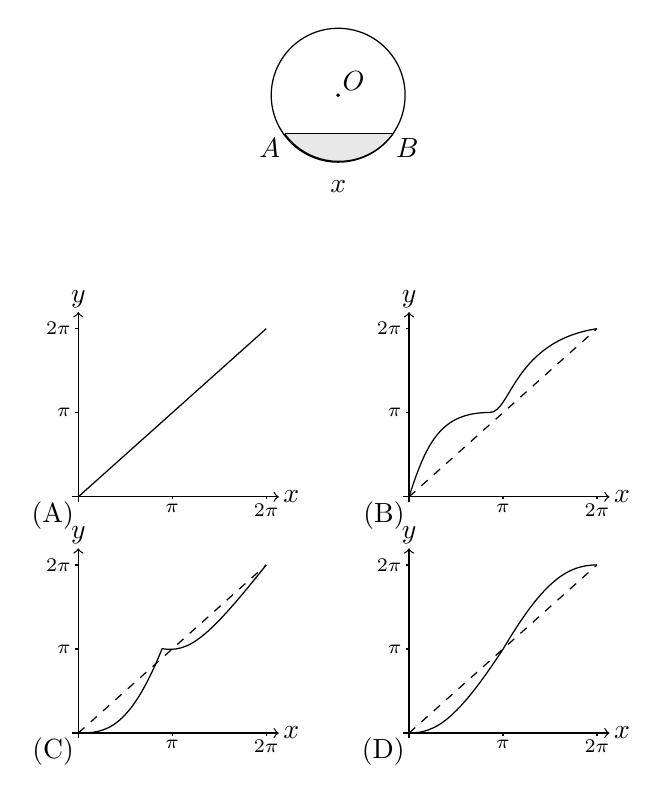
\begin{tikzpicture}[line width=0.45pt,every node/.style={inner sep=1.4pt}]
% Source circle, chord AB, shaded circular segment, center O and arc-length label x.
\begin{scope}[xshift=3.3cm,yshift=5.1cm]
 \draw (0,0) circle (0.85);
 \coordinate (A) at (-0.68,-0.49); \coordinate (B) at (0.68,-0.49);
 \fill[gray!18] (A) arc[start angle=216,end angle=324,radius=0.85] -- (B) -- cycle;
 \draw (A) arc[start angle=216,end angle=324,radius=0.85]; \draw (A)--(B);
 \fill (0,0) circle (0.025) node[above right] {$O$};
 \node[below left] at (A) {$A$}; \node[below right] at (B) {$B$}; \node[below] at (0,-1.03) {$x$};
\end{scope}
% Four graph options in a 2 by 2 layout. The dashed y=x reference is visible in B,C,D.
% Each coordinate system represents x,y from 0 to 2pi; curves are qualitative sketches.
\begin{scope}[xshift=0cm,yshift=0cm,x=0.38cm,y=0.34cm]
 \draw[->] (-0.2,0)--(6.7,0) node[right] {$x$}; \draw[->] (0,-0.2)--(0,6.9) node[above] {$y$};
 \draw (0,0)--(6.28,6.28); \node[below left] at (0,0) {(A)};
 \foreach \t/\lab in {3.14/\pi,6.28/2\pi} {\draw (\t,0)--(\t,-0.1) node[below] {\scriptsize $\lab$}; \draw (0,\t)--(-0.1,\t) node[left] {\scriptsize $\lab$};}
\end{scope}
\begin{scope}[xshift=4.2cm,yshift=0cm,x=0.38cm,y=0.34cm]
 \draw[->] (-0.2,0)--(6.7,0) node[right] {$x$}; \draw[->] (0,-0.2)--(0,6.9) node[above] {$y$};
 \draw[dashed] (0,0)--(6.28,6.28); \draw (0,0) .. controls (0.6,2.1) and (1.1,3.15) .. (2.7,3.15) .. controls (3.4,3.15) and (3.5,5.8) .. (6.28,6.28); \node[below left] at (0,0) {(B)};
 \foreach \t/\lab in {3.14/\pi,6.28/2\pi} {\draw (\t,0)--(\t,-0.1) node[below] {\scriptsize $\lab$}; \draw (0,\t)--(-0.1,\t) node[left] {\scriptsize $\lab$};}
\end{scope}
\begin{scope}[xshift=0cm,yshift=-3.0cm,x=0.38cm,y=0.34cm]
 \draw[->] (-0.2,0)--(6.7,0) node[right] {$x$}; \draw[->] (0,-0.2)--(0,6.9) node[above] {$y$};
 \draw[dashed] (0,0)--(6.28,6.28); \draw (0,0) .. controls (0.9,0) and (1.7,0.1) .. (2.8,3.15) .. controls (3.7,3.0) and (4.3,3.5) .. (6.28,6.28); \node[below left] at (0,0) {(C)};
 \foreach \t/\lab in {3.14/\pi,6.28/2\pi} {\draw (\t,0)--(\t,-0.1) node[below] {\scriptsize $\lab$}; \draw (0,\t)--(-0.1,\t) node[left] {\scriptsize $\lab$};}
\end{scope}
\begin{scope}[xshift=4.2cm,yshift=-3.0cm,x=0.38cm,y=0.34cm]
 \draw[->] (-0.2,0)--(6.7,0) node[right] {$x$}; \draw[->] (0,-0.2)--(0,6.9) node[above] {$y$};
 \draw[dashed] (0,0)--(6.28,6.28); \draw (0,0) .. controls (0.9,0) and (1.6,0.5) .. (3.15,3.15) .. controls (4.4,5.5) and (5.2,6.28) .. (6.28,6.28); \node[below left] at (0,0) {(D)};
 \foreach \t/\lab in {3.14/\pi,6.28/2\pi} {\draw (\t,0)--(\t,-0.1) node[below] {\scriptsize $\lab$}; \draw (0,\t)--(-0.1,\t) node[left] {\scriptsize $\lab$};}
\end{scope}
\end{tikzpicture}
\end{center}
\nopagebreak[4]
\Needspace{4\baselineskip}
\textbf{解析}

单位圆中弧长 \(x\) 就是圆心角（弧度），其中 \(0\le x\le2\pi\)。弓形面积等于扇形面积减去三角形面积：\(x/2-\sin x/2\)。题设取面积的两倍，故 \(f(x)=x-\sin x\)。有 \(f'(x)=1-\cos x\ge0\)，且 \(f''(x)=\sin x\)：在 \((0,\pi)\) 上图像向上弯，在 \((\pi,2\pi)\) 上向下弯。端点处 \(f(0)=0\)、\(f(2\pi)=2\pi\)。符合这些性质的图象为 D。

\gkanswer{答案：D。}

\end{answer}
\begin{answer}
\gksolhead{10}{}

\textbf{题目}：

若 \(a,b,c>0\) 且 \(a(a+b+c)+bc=4-2\sqrt3\)，则 \(2a+b+c\) 的最小值为（　）

(A) \(\sqrt3-1\)　(B) \(\sqrt3+1\)　(C) \(2\sqrt3+2\)　(D) \(2\sqrt3-2\)

\Needspace{4\baselineskip}
\textbf{解析}

\Needspace{5\baselineskip}
令 \(u=a+b\)、\(v=a+c\)，则 \(u,v>0\)，并且
\nopagebreak[4]
\[
uv=(a+b)(a+c)=a(a+b+c)+bc=4-2\sqrt3=(\sqrt3-1)^2.
\]
目标量为 \(2a+b+c=u+v\)。由均值不等式，\(u+v\ge2\sqrt{uv}=2(\sqrt3-1)\)，等号在 \(u=v=\sqrt3-1\) 时成立。该等号可实现：取正的 \(a\) 充分小，并令 \(b=c=\sqrt3-1-a>0\)，则乘积条件成立。因此最小值为 \(2\sqrt3-2\)，选 D。

\gkanswer{答案：D，2√3$-$2。}

\end{answer}
\begin{answer}
\gksolhead{11}{}

\textbf{题目}：

复数 \(\dfrac{1+2i}{3+i^3}\) 的值是\gkblank{}。

\Needspace{4\baselineskip}
\textbf{解析}

\Needspace{5\baselineskip}
因为 \(i^3=-i\)，分母为 \(3-i\)。分子分母同乘共轭复数 \(3+i\)：
\nopagebreak[4]
\[
\frac{1+2i}{3-i}=\frac{(1+2i)(3+i)}{(3-i)(3+i)}=\frac{1+7i}{10}.
\]

\gkanswer{答案：(1+7i)/10。}

\end{answer}
\begin{answer}
\gksolhead{12}{}

\textbf{题目}：

\(\displaystyle\lim_{n\to\infty}\frac{1+3+\cdots +(2n-1)}{2n^2-n+1}=\)\gkblank{}。

\Needspace{4\baselineskip}
\textbf{解析}

\Needspace{5\baselineskip}
前 \(n\) 个正奇数之和为 \(n^2\)，故原式为
\nopagebreak[4]
\[
\frac{n^2}{2n^2-n+1}=\frac1{2-1/n+1/n^2}\longrightarrow\frac12.
\]

\gkanswer{答案：1/2。}

\end{answer}
\begin{answer}
\gksolhead{13}{}

\textbf{题目}：

已知 \(\alpha,\beta\in\left(\dfrac{3\pi}{4},\pi\right)\)，\(\sin(\alpha+\beta)=-\dfrac35\)，\(\sin\left(\beta-\dfrac\pi4\right)=\dfrac{12}{13}\)，则 \(\cos\left(\alpha+\dfrac\pi4\right)=\)\gkblank{}。

\Needspace{4\baselineskip}
\textbf{解析}

\Needspace{5\baselineskip}
令 \(u=\beta-\pi/4\)。由 \(\beta\in(3\pi/4,\pi)\)，有 \(u\in(\pi/2,3\pi/4)\)，故 \(\sin u=12/13\)、\(\cos u=-5/13\)。又 \(\alpha+\beta\in(3\pi/2,2\pi)\)，且其正弦为 \(-3/5\)，所以余弦为 \(4/5\)。
\nopagebreak[4]
\[
\cos(\alpha+\pi/4)=\cos((\alpha+\beta)-u)
=\frac45\left(-\frac5{13}\right)+\left(-\frac35\right)\frac{12}{13}=-\frac{56}{65}.
\]

\gkanswer{答案：$-$56/65。}

\end{answer}
\begin{answer}
\gksolhead{14}{}

\textbf{题目}：

在数列 \(\{a_n\}\) 中，若 \(a_1=1\)，\(a_{n+1}=2a_n+3\ (n\geq1)\)，则该数列的通项 \(a_n=\)\gkblank{}。

\Needspace{4\baselineskip}
\textbf{解析}

令 \(b_n=a_n+3\)，则 \(b_{n+1}=a_{n+1}+3=2a_n+6=2b_n\)，且 \(b_1=4\)。于是 \(b_n=4\cdot2^{n-1}=2^{n+1}\)，从而 \(a_n=2^{n+1}-3\)。

\gkanswer{答案：aₙ=2ⁿ⁺¹$-$3。}

\end{answer}
\begin{answer}
\gksolhead{15}{}

\textbf{题目}：

设 \(a>0\)，\(a\ne1\)，函数 \(f(x)=a^{\lg(x^2-2x+3)}\) 有最大值，则不等式 \(\log_a(x^2-5x+7)>0\) 的解集为\gkblank{}。

\Needspace{4\baselineskip}
\textbf{解析}

令 \(q(x)=x^2-2x+3=(x-1)^2+2\)，其取值范围是 \([2,\infty)\)。若 \(a>1\)，则 \(a^{\lg q(x)}\) 随 \(q(x)\) 严格增大而无上界；若 \(0<a<1\)，它随 \(q(x)\) 增大而递减，并在 \(q=2\) 处取得最大值。因此最大值存在迫使 \(0<a<1\)。底数在此范围内时，\(\log_a t>0\) 等价于 \(0<t<1\)。令 \(t=x^2-5x+7\)，解 \(x^2-5x+7<1\)，即 \((x-2)(x-3)<0\)，得到 \(2<x<3\)。

\gkanswer{答案：(2,3)。}

\end{answer}
\begin{answer}
\gksolhead{16}{}

\textbf{题目}：

已知变量 \(x,y\) 满足约束条件 \(1\leq x+y\leq4\)，\(-2\leq x-y\leq2\)。若目标函数 \(z=ax+y\)（其中 \(a>0\)）仅在点 \((3,1)\) 处取得最大值，则 \(a\) 的取值范围为\gkblank{}。

\Needspace{4\baselineskip}
\textbf{解析}

\Needspace{5\baselineskip}
设 \(u=x+y\)、\(v=x-y\)，约束成为矩形 \(1\le u\le4\)、\(-2\le v\le2\)，而目标函数为
\nopagebreak[4]
\[
z=ax+y=\frac{a+1}{2}u+\frac{a-1}{2}v.
\]
点 \((x,y)=(3,1)\) 对应 \((u,v)=(4,2)\)。因 \(a>0\)，\(u\) 的系数恒正，唯一最大要求 \(v\) 的系数也严格为正；若系数为零则整条边都取最大，若为负则最大点在 \(v=-2\)。故须且只须 \(a>1\)。

\gkanswer{答案：a>1。}

\end{answer}
\begin{answer}
\gksolhead{17}{}

\textbf{题目}：

设函数 \(f(x)=\sqrt3\cos^2\omega x+\sin\omega x\cos\omega x+a\)（其中 \(\omega>0\)，\(a\in\mathbb R\)），且 \(f(x)\) 的图象在 \(y\) 轴右侧的第一个最高点的横坐标为 \(\dfrac\pi6\)。

(1) 求 \(\omega\) 的值；

(2) 如果 \(f(x)\) 在区间 \(\left[-\dfrac\pi3,\dfrac{5\pi}6\right]\) 上的最小值为 \(\sqrt3\)，求 \(a\) 的值。

\Needspace{4\baselineskip}
\textbf{解析}

\gksubpart{(1) 求 \(\omega\)}

\Needspace{5\baselineskip}
利用倍角恒等式，函数可写成
\nopagebreak[4]
\[
f(x)=\frac{\sqrt3}{2}+a+\cos(2\omega x-\pi/6).
\]
其最高点满足 \(2\omega x-\pi/6=2k\pi\)，横坐标为 \(x=\pi/(12\omega)+k\pi/\omega\)。因 \(\omega>0\)，在 \(y\) 轴右侧第一个最高点对应 \(k=0\)。于是 \(\pi/(12\omega)=\pi/6\)，得 \(\omega=1/2\)。

\gksubpart{(2) 求 \(a\)}

代入 \(\omega=1/2\)，余弦相位在给定区间随 \(x\) 从 \(-\pi/2\) 变化至 \(2\pi/3\)。给定相位区间上余弦的最小值为 \(-1/2\)，在右端点取到。因此函数最小值为 \(\sqrt3/2+a-1/2\)。令其等于 \(\sqrt3\)，得到 \(a=(\sqrt3+1)/2\)。

\gkanswer{答案（1）：ω=1/2。}

\gkanswer{答案（2）：a=(√3+1)/2。}

\end{answer}
\begin{answer}
\gksolhead{18}{}

\textbf{题目}：

某大厦的一部电梯从底层出发后只能在第 18、19、20 层可以停靠。若该电梯在底层载有 5 位乘客，且每位乘客在这三层的每一层下电梯的概率均为 \(\dfrac13\)，用 \(\xi\) 表示这 5 位乘客在第 20 层下电梯的人数，求：

(1) 随机变量 \(\xi\) 的分布列；

(2) 随机变量 \(\xi\) 的期望。

\Needspace{4\baselineskip}
\textbf{解析}

\gksubpart{(1) 分布列}

\Needspace{5\baselineskip}
每位乘客在第 20 层下电梯的概率为 \(1/3\)，5 位乘客的选择相互独立。因此 \(\xi\) 是 5 次独立伯努利试验中成功次数，且
\nopagebreak[4]
\[
\Pr(\xi=k)=\binom5k\left(\frac13\right)^k\left(\frac23\right)^{5-k},\qquad k=0,1,2,3,4,5.
\]

\gksubpart{(2) 期望}

二项分布 \(\operatorname{Bin}(5,1/3)\) 的期望为试验次数乘成功概率，故 \(\mathbb E\xi=5/3\)。

\gkanswer{答案（1）：ξ~Bin(5,1/3)，P(ξ=k)=C(5,k)(1/3)^k(2/3)^(5$-$k)，k=0,…,5。}

\gkanswer{答案（2）：Eξ=5/3。}

\end{answer}
\begin{answer}
\gksolhead{19}{}

\textbf{题目}：

如图，在四棱锥 \(P-ABCD\) 中，\(PA\perp\) 底面 \(ABCD\)，\(\angle DAB\) 为直角，\(AB\parallel CD\)，\(AD=CD=2AB\)，\(E、F\) 分别为 \(PC、CD\) 的中点。
\nopagebreak[4]
\begin{center}% Source-faithful schematic draft: 2006 Chongqing Science Q19, PDF p.2 (printed p.285).
% Source ID: src-5abd831561d7d4fa968c5bf0deb634e0d666376fd8cc90967cf30d301e77a351
% Source SHA-256: 211d79b8676187c7e4a98c71d7eae5eadd28b2e5aaf9237fefd55a791241faa3
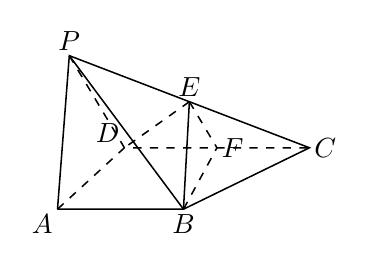
\begin{tikzpicture}[line width=0.55pt,every node/.style={inner sep=1.5pt}]
 % The base is shown in oblique projection; dashed segments reproduce hidden edges in the source.
 \coordinate (A) at (0,0); \coordinate (B) at (1.6,0); \coordinate (D) at (0.85,0.78); \coordinate (C) at (3.2,0.78); \coordinate (P) at (0.15,1.95);
 \coordinate (E) at (1.675,1.365); % E is the projected midpoint of PC
 \coordinate (F) at (2.025,0.78); % midpoint of CD in the drawn projection
 \draw (A)--(B)--(C)--(P)--(A);
 \draw (P)--(B);
 \draw[dashed] (A)--(D)--(C);
 \draw[dashed] (P)--(D);
 \draw (E)--(B);
 \draw[dashed] (E)--(D) (E)--(F) (B)--(F);
 \foreach \pt/\pos/\lab in {A/below left/A,B/below/B,C/right/C,D/above left/D,P/above/P,E/above/E,F/right/F}
   \node[\pos] at (\pt) {$\lab$};
\end{tikzpicture}
\end{center}
\nopagebreak[4]
(1) 试证：\(CD\perp\) 平面 \(BEF\)；

(2) 设 \(PA=k\cdot AB\)，且二面角 \(E-BD-C\) 的平面角大于 \(30^\circ\)，求 \(k\) 的取值范围。

\Needspace{4\baselineskip}
\textbf{解析}

\gksubpart{(1) 证明 \(CD\perp\) 平面 \(BEF\)}

设 \(AB=s>0\)。取直角坐标系令 \(A=(0,0,0)\)，\(B=(s,0,0)\)，\(D=(0,2s,0)\)。由 \(AB\parallel CD\)、\(CD=2s\) 且四边形为四棱锥底面，按题面几何次序可取 \(C=(2s,2s,0)\)；又 \(PA\perp\) 底面，记 \(P=(0,0,h)\)，其中 \(h>0\)。中点坐标为 \(E=(s,s,h/2)\)、\(F=(s,2s,0)\)。方向向量 \(\overrightarrow{CD}=(-2s,0,0)\)，\(\overrightarrow{BE}=(0,s,h/2)\)，\(\overrightarrow{BF}=(0,2s,0)\)。后两向量均与 \(CD\) 垂直，且不共线，故它们张成平面 \(BEF\)，从而 \(CD\perp\) 平面 \(BEF\)。

\gksubpart{(2) 求 \(k\) 的范围}

\Needspace{5\baselineskip}
作垂直于 \(BD\) 的截面，截面分别与平面 \(EBD\)、底面 \(CBD\) 相交于两条射线，其夹角即二面角的平面角 \(\theta\)。取 \(s=1\)，有 \(\overrightarrow{BD}=(-1,2,0)\)、\(\overrightarrow{BE}=(0,1,k/2)\)。平面 \(EBD\) 的法向量可取
\nopagebreak[4]
\[
\overrightarrow{BD}\times\overrightarrow{BE}=(k,k/2,-1),
\]
\Needspace{5\baselineskip}
底面法向量为 \((0,0,1)\)。由截面角的余弦（取两平面所成的锐角）得
\nopagebreak[4]
\[
\cos\theta=\frac1{\sqrt{1+5k^2/4}}.
\]
题设 \(\theta>30^\circ\) 等价于 \(\cos\theta<\sqrt3/2\)，故 \(1+5k^2/4>4/3\)，即 \(k^2>4/15\)。因 \(PA=k\cdot AB\) 且 \(PA,AB>0\)，所以 \(k>0\)，最终 \(k>2/\sqrt{15}\)。

\gkanswer{答案（1）：CD$\perp$平面 BEF。}

\gkanswer{答案（2）：k>2/√15。}

\end{answer}
\begin{answer}
\gksolhead{20}{}

\textbf{题目}：

已知函数 \(f(x)=(x^2+bx+c)e^x\)，其中 \(b,c\in\mathbb R\) 为常数。

(1) 若 \(b^2>4(a-1)\)，讨论函数 \(f(x)\) 的单调性；

(2) 若 \(b^2\leq4(c-1)\)，且 \(\displaystyle\lim_{x\to0}\frac{f(x)-c}{x}=4\)，试证：\(-6\leq b\leq2\)。

\begin{gktip}
\textbf{原文存疑}：函数定义中参数为 $b,c$，但 Q20(1) 固定原页印作 $b^2>4(a-1)$。此处照录可见字母 $a$，不推测改成 $c$。
\end{gktip}

\Needspace{4\baselineskip}
\textbf{解析}

\gksubpart{(1) 单调性}

题面明文条件为 \(b^2>4(a-1)\)，而函数定义只引入参数 \(b,c\)，没有定义 \(a\)。故当前原文不能确定该不等式对 \(b,c\) 的限制，无法唯一确定导数零点和单调区间。本小问保留 U/PENDING；在题面疑点澄清前不作猜测性更正或求解。

\gksubpart{(2) 证明 \(-6\le b\le2\)}

\Needspace{5\baselineskip}
由 \(f(0)=c\)，且 \(f'(0)=c+b\)，给定极限就是 \(f'(0)=4\)，故 \(b+c=4\)，即 \(c=4-b\)。将其代入 \(b^2\le4(c-1)\)，得
\nopagebreak[4]
\[
b^2\le4(3-b)\quad\Longleftrightarrow\quad b^2+4b-12\le0
\quad\Longleftrightarrow\quad(b+6)(b-2)\le0.
\]
因此 \(-6\le b\le2\)。

\gkanswer{答案（1）：U/PENDING。}

\gkanswer{答案（2）：$-$6≤b≤2。}

\end{answer}
\begin{answer}
\gksolhead{21}{}

\textbf{题目}：

已知定义域为 \(\mathbb R\) 的函数 \(f(x)\) 满足 \(f(f(x)-x^2+x)=f(x)-x^2+x\)。

(1) 若 \(f(2)=3\)，求 \(f(1)\)；又若 \(f(0)=a\)，求 \(f(a)\)；

(2) 设有且仅有一个实数 \(x_0\)，使得 \(f(x_0)=x_0\)，求函数 \(f(x)\) 的解析表达式。

\Needspace{4\baselineskip}
\textbf{解析}

\gksubpart{(1) 求函数值}

令 \(g(x)=f(x)-x^2+x\)。题设关系成为 \(f(g(x))=g(x)\)，即每个 \(g(x)\) 都是 \(f\) 的不动点。先由 \(f(2)=3\) 得 \(g(2)=3-4+2=1\)，所以 \(f(1)=1\)。再令 \(f(0)=a\)，则 \(g(0)=a\)，因此 \(f(a)=a\)。

\gksubpart{(2) 确定解析式}

\Needspace{5\baselineskip}
由 (1) 中的恒等关系，对任意实数 \(x\)，\(g(x)=f(x)-x^2+x\) 是不动点。题设不动点恰有一个，记为 \(x_0\)，于是对所有 \(x\)，\(g(x)=x_0\)，即
\nopagebreak[4]
\[
f(x)=x^2-x+x_0.
\]
不动点需满足 \(x^2-x+x_0=x\)，即 \(x^2-2x+x_0=0\)。此方程恰有一个实根，判别式为零：\(4-4x_0=0\)，所以 \(x_0=1\)。故 \(f(x)=x^2-x+1\)。

\gkanswer{答案（1）：f(1)=1，f(a)=a。}

\gkanswer{答案（2）：f(x)=x²$-$x+1。}

\end{answer}
\begin{answer}
\gksolhead{22}{}

\textbf{题目}：

已知一列椭圆 \(C_n:x^2+\dfrac{y^2}{b_n^2}=1\)，\(0<b_n<1\)，\(n=1,2,\cdots\)。若椭圆 \(C_n\) 上有一点 \(P_n\)，使 \(P_n\) 到右准线 \(l_n\) 的距离 \(d_n\) 是 \(|P_nF_n|\) 与 \(|P_nG_n|\) 的等差中项，其中 \(F_n、G_n\) 分别是 \(C_n\) 的左、右焦点。
\nopagebreak[4]
\begin{center}% Source-faithful schematic draft: 2006 Chongqing Science Q22, PDF p.2 (printed p.285).
% Source ID: src-5abd831561d7d4fa968c5bf0deb634e0d666376fd8cc90967cf30d301e77a351
% Source SHA-256: 211d79b8676187c7e4a98c71d7eae5eadd28b2e5aaf9237fefd55a791241faa3
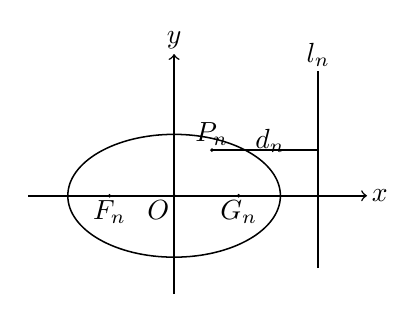
\begin{tikzpicture}[x=1cm,y=1cm,line width=0.55pt,every node/.style={inner sep=1.5pt}]
 % Ellipse, coordinate axes, right directrix l_n, point P_n, foci and horizontal distance d_n.
 \draw (0,0) ellipse (1.35 and 0.78);
 \draw[->] (-1.85,0)--(2.45,0) node[right] {$x$};
 \draw[->] (0,-1.25)--(0,1.8) node[above] {$y$};
 \draw (1.83,-0.92)--(1.83,1.58) node[above] {$l_n$};
 \coordinate (Pn) at (0.48,0.58); \coordinate (Fn) at (-0.82,0); \coordinate (Gn) at (0.82,0);
 \fill (Pn) circle (0.025) node[above] {$P_n$};
 \fill (Fn) circle (0.025) node[below] {$F_n$};
 \fill (Gn) circle (0.025) node[below] {$G_n$};
 \fill (0,0) circle (0.025) node[below left] {$O$};
 \draw (Pn)--(1.83,0.58);
 \node at (1.22,0.70) {$d_n$};
\end{tikzpicture}
\end{center}
\nopagebreak[4]
(1) 试证：\(b_n\leq\dfrac{\sqrt3}{2}\ (n\geq1)\)；

(2) 取 \(b_n=\dfrac{\sqrt{2n+3}}{n+2}\)，并用 \(S_n\) 表示 \(\triangle P_nF_nG_n\) 的面积，试证：\(S_1<S_2\) 且 \(S_n>S_{n+1}\ (n\geq3)\)。

\Needspace{4\baselineskip}
\textbf{解析}

\Needspace{5\baselineskip}
记某椭圆的半长轴为 1、半短轴为 \(b\)，焦距参数 \(c=\sqrt{1-b^2}\)，于是左右焦点为 \((-c,0),(c,0)\)，右准线为 \(x=1/c\)。椭圆上任一点到两焦点距离之和为 2。题设说到右准线的距离是两焦距的等差中项，即为两焦距的算术平均，因此该距离等于 1。设点 \(P=(x,y)\)，则
\nopagebreak[4]
\[
\frac1c-x=1,\qquad x=\frac1c-1.
\]

\gksubpart{(1) 证明 \(b_n\le\sqrt3/2\)}

椭圆上点的横坐标满足 \(x\le1\)。上式于是给出 \(1/c-1\le1\)，即 \(c\ge1/2\)。因为 \(b^2=1-c^2\)，所以 \(b^2\le3/4\)，结合 \(b>0\) 得 \(b\le\sqrt3/2\)。该推导逐项适用于每个 \(n\)。

\gksubpart{(2) 证明面积大小关系}

\Needspace{5\baselineskip}
给定 \(b_n=\sqrt{2n+3}/(n+2)\)，计算
\nopagebreak[4]
\[
c_n=\sqrt{1-b_n^2}=\frac{n+1}{n+2},\qquad x_n=\frac1{c_n}-1=\frac1{n+1}.
\]
\Needspace{5\baselineskip}
从椭圆方程得 \(y_n^2=b_n^2(1-x_n^2)\)。三角形 \(P_nF_nG_n\) 的底边长为 \(2c_n\)，高为 \(|y_n|\)，因此 \(S_n=c_n|y_n|\)，且
\nopagebreak[4]
\[
S_n^2=c_n^2b_n^2(1-x_n^2)
=\frac{n(2n+3)}{(n+2)^3}.
\]
\Needspace{5\baselineskip}
面积非负，比较平方即可。先算得 \(S_1^2=5/27\)、\(S_2^2=7/32\)，且 \(7/32-5/27=29/864>0\)，故 \(S_1<S_2\)。对 \(n\ge3\)，相邻平方差通分为
\nopagebreak[4]
\[
S_n^2-S_{n+1}^2
=\frac{2n^4+10n^3+5n^2-35n-40}{(n+2)^3(n+3)^3}.
\]
\Needspace{5\baselineskip}
分母为正。记分子为 \(p(n)\)，有 \(p(3)=332>0\)，且对整数 \(n\ge3\)，
\nopagebreak[4]
\[
p(n+1)-p(n)=8n^3+42n^2+48n-18>0.
\]
所以分子对 \(n\ge3\) 始终为正，得到 \(S_n^2>S_{n+1}^2\)，即 \(S_n>S_{n+1}\)。

\gkanswer{答案（1）：bₙ≤√3/2。}

\gkanswer{答案（2）：S₁<S₂ 且 Sₙ>Sₙ₊₁（n≥3）。}

\end{answer}